The lolly machine is a demonstration unit for Murdoch University Engineering that sorts and dispenses Lollies as according to colour. The intended purpose of the lolly machine is to spark the interest of future engineering students during open days and to showcase the capabilities of \acrlong{icse} students.

The lolly machine has been out of service for some time and is in desperate need of maintenance and an upgrade. The thesis project aligned with this document has two fundamental aims. The first is to get the lolly machine back to an operable state. The second is to upgrade the control system to bring it inline with modern-day technologies. As this is the second upgrade that the machine has seen the project has been named, \textbf{The Lolly Machine Upgrade 2}.

Given the nature of this thesis project a literature review is not applicable - this document will serve more as a background rather than a literature review.

This document aims to preface the reader, giving them the necessary knowledge base required to understand the concepts and terms used throughout the main body of the proceeding thesis report.

    \begin{figure}[ht]
        \centering
        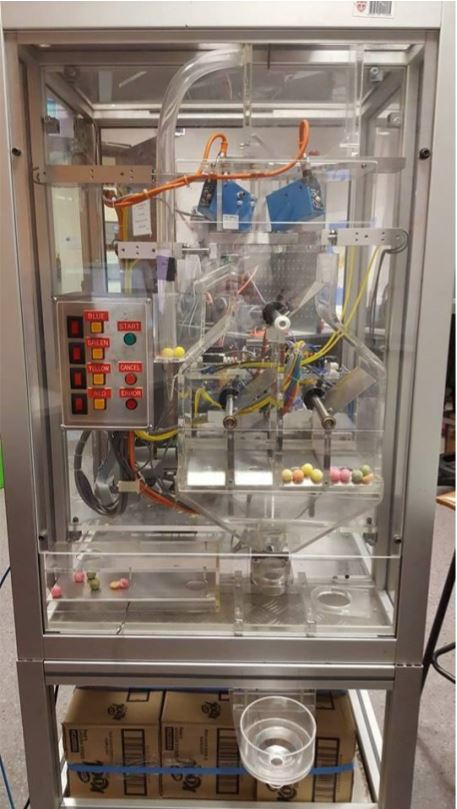
\includegraphics[scale = 0.5]{lollyMachine.JPG}
        \caption{The lolly machine~\cite{thesisJodie}.}
        \label{fig:lollyMachine}
    \end{figure}
